\documentclass{beamer}
\usetheme{Warsaw}
\useinnertheme{circles}
\useoutertheme[subsection=false]{smoothbars}
\usepackage[utf8x]{inputenc}
\usepackage[czech]{babel}
\usepackage[T1]{fontenc}
\usepackage{listings}
\usepackage{tikz}
\lstset{basicstyle=\tiny\ttfamily}
\logo{
\includegraphics[height=0.5cm]{brmlab.pdf}}

\begin{document}

\AtBeginSection[]
{
  \begin{frame}
    \frametitle{Outline}
    \tableofcontents[currentsection]
  \end{frame}
}

\title{brmiversity: Umělá inteligence \\ a teoretická informatika}
\subtitle{Přednáška č. 10}
\author{Petr Baudiš $\langle${\tt pasky@ucw.cz}$\rangle$}
\institute{
	brmlab 2011\\
	\vskip 1ex
	\pgfdeclareimage[height=4ex]{ccbysa}{by-sa.pdf}
	\pgfuseimage{ccbysa}
}
\date{}
\frame{\titlepage}

\section{Umělá inteligence a adaptivní agenti}

\subsection{}
\begin{frame}{Strojové učení}
\begin{center}
Učící se agent: Datový vstup a výstup, rozhodovací problém, užitková funkce
\vskip 3ex
\begin{block}{Máme trénovací množinu}
\begin{itemize}
\item Učení s učitelem vs. bez učitele
\item Rozpoznávání vs. samoorganizace
\end{itemize}
\end{block}
\begin{block}{Nemáme trénovací množinu}
\begin{itemize}
\item Exploration---exploitation dilemma
\item Zpětnovazebné učení
\end{itemize}
\end{block}
\end{center}
\end{frame}

\subsection{}
\begin{frame}{Strojové učení zkušeností}
\begin{center}
Dnes: Data si musíme shánět sami průběžně.

\vskip 3ex

Musíme přitom již co nejlépe fungovat. \\
(Nenechat se zabít, dělat něco užitečného.)

\vskip 3ex

Učit se chceme co nejefektivněji.

\vskip 3ex

Problém výběru akcí --- zase! \\
Exploration: Data o alternativách. \\
Exploitation: Výběr nejlepší alternativy. \\
Exploration a exploitation jsou v opozici natrvalo.
\end{center}
\end{frame}

\subsection{}
\begin{frame}{Zpětnovazebné učení}
\begin{itemize}
\item Problém mnohorukého loupežníka (multi-armed bandit)
\item Genetický algoritmus
\item Hraní Go
\end{itemize}
\end{frame}

\subsection{}
\begin{frame}{Zpětnovazebné učení}
\begin{itemize}
\item Reinforcement learning
\item Bellmannova rovnice
\item Q-učení
\item atd.
\item Učení neuronových sítí atd. adapt. ag.
\end{itemize}
\end{frame}

\subsection{}
\begin{frame}{Otázky?}
\begin{center}
Příště UI: Reprezentace znalostí.

Příště Adaptivní agenti: Etologie a populační dynamika.
\end{center}
\end{frame}

\section{Neuronové sítě}

\subsection{}
\begin{frame}{Samoorganizace pomocí ANN}
\begin{itemize}
\item Umělé neurony (``výpočetní krabičky'') \\ dostávají vstupy (čísla) a na jejich \\ základě generují výstup (číslo)
\item Dnes: Chceme asociovat různé vstupy s různými neurony
\end{itemize}
\begin{tikzpicture}[remember picture,overlay]
  \node [xshift=-4.5cm,yshift=-4.5cm,above right] at (current page.north east)
    {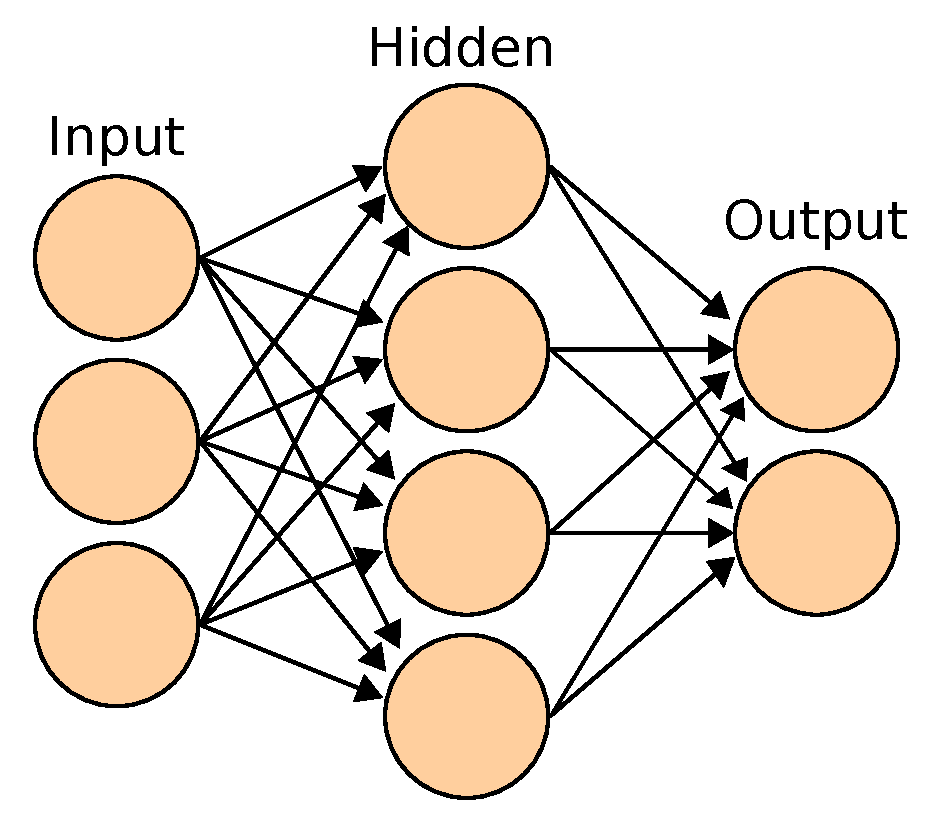
\includegraphics[width=4cm]{ANN.pdf}};
\end{tikzpicture}
\end{frame}

\subsection{}
\begin{frame}{Kohonenova mapa}
\begin{itemize}
\item Fonetický psací stroj, ekonomická data
\item Organizace, princip, učení
\item XXX: nebo jindy?!
\end{itemize}
\end{frame}

\subsection{}
\begin{frame}{Ojův algoritmus}
\begin{itemize}
\item PCA pomocí ANN
\end{itemize}
\end{frame}

\subsection{}
\begin{frame}{Další metody samoorganizace}
\begin{itemize}
\item Laterální inhibice, ART, RBF
\end{itemize}
\end{frame}

\subsection{}
\begin{frame}{Otázky?}
\begin{center}
Příště: ??
\end{center}
\end{frame}

\section{Datové struktury}

\subsection{}
\begin{frame}{Haldy}
\begin{itemize}
\item Rekapitulace.
\item Levicová halda.
\item Binomiální a Fibonacciho haldy.
\end{itemize}
\end{frame}

\subsection{}
\begin{frame}{B-stromy}
\begin{itemize}
\item Co to je, jak se to chová
\item Vlastnosti
\item Vyvažování
\end{itemize}
\end{frame}

\subsection{}
\begin{frame}{Otázky?}
\begin{center}
Příště: Datové struktury v externí paměti.
\end{center}
\end{frame}

\subsection{}
\begin{frame}{Děkuji vám}
\begin{center}
{\bf pasky@ucw.cz}

\vskip 6ex

Příště: Neuronové sítě.
	Adaptivní agenti.
	Evoluční algoritmy (koevoluce, otevřená evoluce, teoretická analýza). \\
	Složitost (vlastnosti tříd složitosti).
\end{center}
\end{frame}

\end{document}
